\documentclass[aspectratio=169, 11pt]{beamer}

% ── Theme: same clean white style as the Project 1 slides ──
\usetheme{default}
\usecolortheme{default}
\setbeamercolor{structure}{fg=black!80}
\setbeamercolor{frametitle}{fg=black!90, bg=white}
\setbeamercolor{title}{fg=black!90}
\setbeamercolor{subtitle}{fg=black!60}
\setbeamercolor{author}{fg=black!70}
\setbeamercolor{normal text}{fg=black!85, bg=white}
\setbeamercolor{block title}{fg=white, bg=black!70}
\setbeamercolor{block body}{fg=black!85, bg=black!5}
\setbeamercolor{block title alerted}{fg=white, bg=red!65!black}
\setbeamercolor{block body alerted}{fg=black!85, bg=red!5}
\setbeamercolor{block title example}{fg=white, bg=green!45!black}
\setbeamercolor{block body example}{fg=black!85, bg=green!5}
\setbeamercolor{itemize item}{fg=black!70}
\setbeamercolor{itemize subitem}{fg=black!60}
\setbeamercolor{enumerate item}{fg=black!70}
\setbeamertemplate{navigation symbols}{}
\setbeamertemplate{footline}{%
  \hfill\insertframenumber/\inserttotalframenumber\hspace*{6pt}\vspace{4pt}%
}
\setbeamertemplate{date}{}
\setbeamerfont{frametitle}{size=\large, series=\bfseries}

% ── Packages ──
\usepackage[utf8]{inputenc}
\usepackage[T1]{fontenc}
\usepackage{amsmath,amssymb}
\usepackage{tikz}
\usetikzlibrary{arrows.meta, positioning, fit, backgrounds, calc}
\usepackage{booktabs}
\usepackage{array}

\tikzset{
  box/.style={draw, rounded corners, align=center, font=\scriptsize,
    minimum width=2.4cm, minimum height=0.6cm},
  arr/.style={-{Stealth[length=1.6mm]}, thick},
  biarr/.style={{Stealth[length=1.6mm]}-{Stealth[length=1.6mm]}, thick},
}

% ── Title info ──
\title{Kubernetes IPAM Efficiency \& CNI Resilience}
\subtitle{CS331 - Computer Networks, Project 2}
\author{
  Arpan Gupta (24110051) \\
  Buha Deep Maheshbhai (24110082) \\
  Param Tanna (24110236) \\
  Ramji Purwar (24110287) \\
  Rathod Yuvraj Rajubhai (24110293) \\
  Solanki Viraj Rajeshbhai (24110348)
}
\date[]{}

\begin{document}

% ───────────────────────── SLIDE 1: Title
\begin{frame}[plain]
  \titlepage
\end{frame}

% ───────────────────────── SLIDE 2: Problem 1
\begin{frame}{Problem 1: Static Pod IP Allocation}
\begin{columns}[c]
\begin{column}{0.46\textwidth}
\footnotesize
Kubernetes gives every node a \textbf{fixed block} of pod addresses (default /24 = 256), once, at creation.
\begin{itemize}
  \item Quiet nodes \alert{waste} most of their block
  \item Busy nodes \alert{run out}: pods stuck in \texttt{ContainerCreating}
  \item The scheduler does not track IPs
  \item No resizing, no growth into a new CIDR, no shrinking
\end{itemize}
\vspace{4pt}
\end{column}
\begin{column}{0.5\textwidth}
\centering
\resizebox{\textwidth}{!}{%
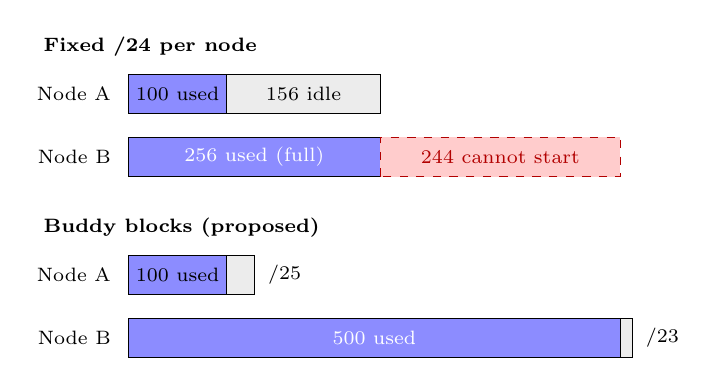
\begin{tikzpicture}[font=\scriptsize, x=1cm, y=1cm]
  \def\s{0.0125}
  \node[anchor=west, font=\scriptsize\bfseries] at (-1.2,1.0) {Fixed /24 per node};
  \node[anchor=east] at (-0.1,0.4) {Node A};
  \draw[fill=blue!45] (0,0.15) rectangle (100*\s,0.65);
  \draw[fill=gray!15] (100*\s,0.15) rectangle (256*\s,0.65);
  \node at (50*\s,0.4) {100 used};
  \node at (178*\s,0.4) {156 idle};
  \node[anchor=east] at (-0.1,-0.4) {Node B};
  \draw[fill=blue!45] (0,-0.65) rectangle (256*\s,-0.15);
  \node[text=white] at (128*\s,-0.4) {256 used (full)};
  \draw[fill=red!20, draw=red!70!black, dashed] (256*\s,-0.65) rectangle (500*\s,-0.15);
  \node[text=red!70!black] at (378*\s,-0.4) {244 cannot start};
  \node[anchor=west, font=\scriptsize\bfseries] at (-1.2,-1.3) {Buddy blocks (proposed)};
  \node[anchor=east] at (-0.1,-1.9) {Node A};
  \draw[fill=blue!45] (0,-2.15) rectangle (100*\s,-1.65);
  \draw[fill=gray!15] (100*\s,-2.15) rectangle (128*\s,-1.65);
  \node at (50*\s,-1.9) {100 used};
  \node[anchor=west] at (128*\s+0.05,-1.9) {/25};
  \node[anchor=east] at (-0.1,-2.7) {Node B};
  \draw[fill=blue!45] (0,-2.95) rectangle (500*\s,-2.45);
  \draw[fill=gray!15] (500*\s,-2.95) rectangle (512*\s,-2.45);
  \node[text=white] at (250*\s,-2.7) {500 used};
  \node[anchor=west] at (512*\s+0.05,-2.7) {/23};
\end{tikzpicture}}
\end{column}
\end{columns}
\end{frame}

% ───────────────────────── SLIDE 3: Solution 1 (IPAM)
\begin{frame}{Solution 1: Buddy-Style Dynamic IPAM}
\begin{columns}[c]
\begin{column}{0.47\textwidth}
\footnotesize
\begin{itemize}
  \item Pool = \textbf{buddy tree}: /22 $\to$ two /23 $\to$ \dots $\to$ /28
  \item Each node gets \textbf{aligned power-of-two blocks}\\ $\Rightarrow$ one route per block
  \item \textbf{Grow} at 80\% use, or at once on\\ ``no IP addresses available''
  \item Prefer the node's \textbf{own buddy} $\Rightarrow$ halves merge
  \item \textbf{Shrink} by draining: no new pods, release when empty; pods never moved
  \item Spill into \textbf{discontiguous} CIDRs, reclaim leaked leases
\end{itemize}
\vspace{4pt}
{\scriptsize Block life: Pending $\to$ Active $\to$ Draining $\to$ Quarantined $\to$ Released}
\end{column}
\begin{column}{0.5\textwidth}
\centering
\resizebox{\textwidth}{!}{%
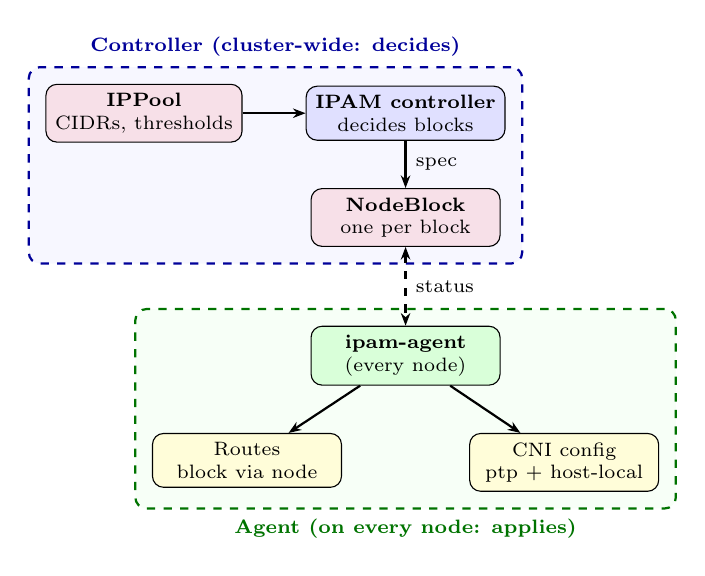
\begin{tikzpicture}
  \node[box, fill=purple!12] (pool) {\textbf{IPPool}\\CIDRs, thresholds};
  \node[box, fill=blue!12, right=0.8cm of pool] (ctrl) {\textbf{IPAM controller}\\decides blocks};
  \node[box, fill=purple!12, below=0.6cm of ctrl] (nb) {\textbf{NodeBlock}\\one per block};
  \node[box, fill=green!15, below=1.0cm of nb] (ag) {\textbf{ipam-agent}\\(every node)};
  \node[box, fill=yellow!15, below left=0.6cm and -0.4cm of ag] (rt) {Routes\\block via node};
  \node[box, fill=yellow!15, below right=0.6cm and -0.4cm of ag] (cfg) {CNI config\\ptp + host-local};
  \draw[arr] (pool) -- (ctrl);
  \draw[arr] (ctrl) -- node[right, font=\scriptsize]{spec} (nb);
  \draw[biarr, dashed] (nb) -- node[right, font=\scriptsize]{status} (ag);
  \draw[arr] (ag) -- (rt);
  \draw[arr] (ag) -- (cfg);
  \begin{scope}[on background layer]
    \node[draw=blue!60!black, thick, dashed, rounded corners, fill=blue!3, fit=(pool)(ctrl)(nb), inner sep=6pt,
      label={[font=\scriptsize\bfseries, text=blue!60!black]north:Controller (cluster-wide: decides)}] {};
    \node[draw=green!45!black, thick, dashed, rounded corners, fill=green!3, fit=(ag)(rt)(cfg), inner sep=6pt,
      label={[font=\scriptsize\bfseries, text=green!45!black]south:Agent (on every node: applies)}] {};
  \end{scope}
\end{tikzpicture}}
\end{column}
\end{columns}
\end{frame}

% ───────────────────────── SLIDE 4: Problem 2
\begin{frame}{Problem 2: The CNI Is a Single Point of Failure}
\begin{columns}[c]
\begin{column}{0.46\textwidth}
\footnotesize
Every pod is \textbf{single-homed}: one interface (\texttt{eth0}), one IP, one path, from one CNI.
\begin{itemize}
  \item CNI data path breaks (routes, tunnel, rules) $\to$ pod \alert{unreachable}
  \item Kubelet uses the \textbf{host network}, so the node still looks \texttt{Ready}
  \item Pods are \alert{not moved}; restarting containers does not fix the network
  \item fix: manual CNI restart or node reboot
\end{itemize}
\vspace{4pt}
No second path, and no way to detect or repair the failure through the network itself.
\end{column}
\begin{column}{0.5\textwidth}
\centering
\resizebox{\textwidth}{!}{%
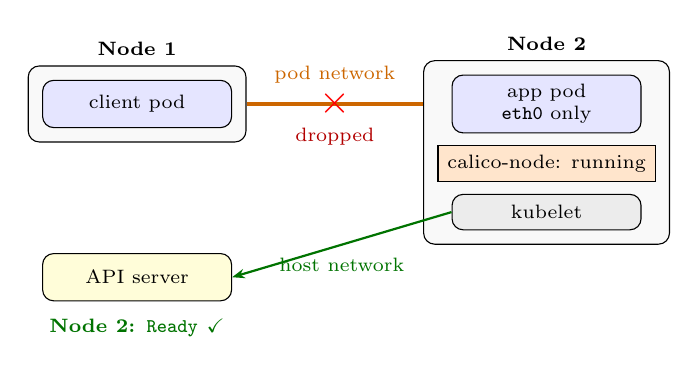
\begin{tikzpicture}[font=\scriptsize]
  % nodes
  \node[box, fill=blue!10] (cli) at (0,0) {client pod};
  \node[box, fill=blue!10] (app) at (5.2,0) {app pod\\\texttt{eth0} only};
  \node[box, fill=orange!20, below=0.15cm of app, rounded corners=0pt, minimum height=0.4cm] (cal) {calico-node: running};
  \node[box, fill=gray!15, below=0.15cm of cal, minimum height=0.45cm] (kl) {kubelet};
  \begin{scope}[on background layer]
    \node[draw, rounded corners, fill=gray!5, fit=(cli), inner sep=5pt,
      label={[font=\scriptsize\bfseries]north:Node 1}] (n1) {};
    \node[draw, rounded corners, fill=gray!5, fit=(app)(cal)(kl), inner sep=5pt,
      label={[font=\scriptsize\bfseries]north:Node 2}] (n2) {};
  \end{scope}
  % broken pod path
  \coordinate (mid) at ($(n1.east |- cli)!0.5!(n2.west |- app)$);
  \draw[very thick, orange!80!black] (n1.east |- cli) -- (n2.west |- app);
  \node[text=orange!80!black, above=4pt] at (mid) {pod network};
  \node[text=red, font=\Large\bfseries] at (mid) {$\times$};
  \node[text=red!70!black, below=5pt] at (mid) {dropped};
  % control path still fine
  \node[box, fill=yellow!15] (api) at (0,-2.2) {API server};
  \draw[thick, green!45!black, -{Stealth[length=1.6mm]}] (kl.west) -- (api.east)
    node[pos=0.5, below=1pt, align=center, text=green!45!black] {host network};
  \node[text=green!45!black, font=\scriptsize\bfseries, below=0.1cm of api] {Node 2: \texttt{Ready} \checkmark};
\end{tikzpicture}}
\end{column}
\end{columns}
\end{frame}

% ───────────────────────── SLIDE 5: Solution 2 (CNI resilience)
\begin{frame}{Solution 2: Dual-CNI Failover}
\begin{columns}[c]
\begin{column}{0.5\textwidth}
\footnotesize
\begin{enumerate}
  \item \textbf{Two paths:} \texttt{eth0} on Calico, \texttt{net1} on Flannel (Multus)
  \item \textbf{Detect:} health agents probe one peer per round over both paths, 3 results in a row to flip
  \item \textbf{Blame:} a node is broken only if probes in \emph{and} out fail while another pair works, else wait
  \item \textbf{Fail over:} readiness gate off ($\texttt{eth0}$ leaves Service) + \textbf{shadow EndpointSlice} with \texttt{net1}
  \item \textbf{Recover:} taint node, restart \texttt{calico-node} once
  \item \textbf{Fail back:} gate on, then delete shadow
\end{enumerate}
\end{column}
\begin{column}{0.47\textwidth}
\centering
\resizebox{\textwidth}{!}{%
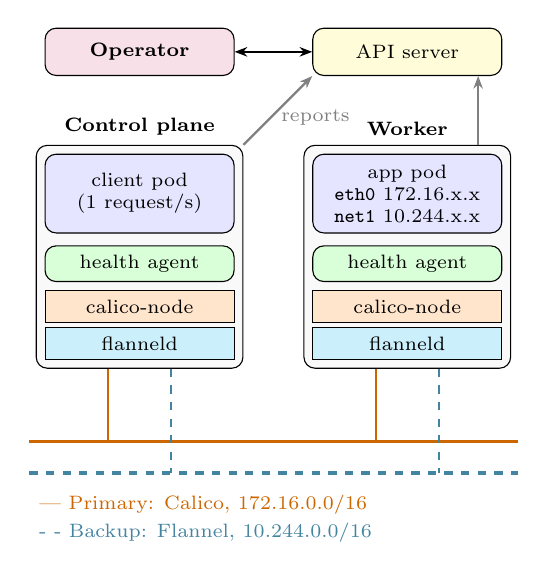
\begin{tikzpicture}[font=\scriptsize]
  \node[box, fill=purple!12] (op) at (0,3.2) {\textbf{Operator}};
  \node[box, fill=yellow!15] (api) at (3.4,3.2) {API server};
  \draw[biarr] (op) -- (api);
  \node[box, fill=blue!10, minimum height=1.0cm] (p1) at (0,1.4) {client pod\\(1 request/s)};
  \node[box, fill=blue!10, minimum height=1.0cm] (p2) at (3.4,1.4) {app pod\\\texttt{eth0} 172.16.x.x\\\texttt{net1} 10.244.x.x};
  \foreach \i/\name in {1/Control plane, 2/Worker} {
    \node[box, fill=green!15, below=0.15cm of p\i, minimum height=0.45cm] (ag\i) {health agent};
    \node[box, fill=orange!20, below=0.1cm of ag\i, minimum height=0.4cm, rounded corners=0pt] (c\i) {calico-node};
    \node[box, fill=cyan!20, below=0.05cm of c\i, minimum height=0.4cm, rounded corners=0pt] (f\i) {flanneld};
    \begin{scope}[on background layer]
      \node[draw, rounded corners, fill=gray!5, fit=(p\i)(f\i), inner sep=3pt,
        label={[font=\scriptsize\bfseries]north:\name}] (n\i) {};
    \end{scope}
  }
  \draw[arr, gray] (n1.north east) -- node[right, pos=0.4]{reports} (api.south west);
  \draw[arr, gray] ([xshift=9mm]n2.north) -- ([xshift=9mm]api.south);
  \draw[very thick, orange!80!black] (-1.4,-1.75) -- (4.8,-1.75);
  \draw[very thick, cyan!60!black, dashed] (-1.4,-2.15) -- (4.8,-2.15);
  \foreach \n in {n1,n2} {
    \draw[orange!80!black, thick] ([xshift=-4mm]\n.south) -- ([xshift=-4mm]\n.south |- 0,-1.75);
    \draw[cyan!60!black, thick, dashed] ([xshift=4mm]\n.south) -- ([xshift=4mm]\n.south |- 0,-2.15);
  }
  \node[anchor=west, orange!80!black] at (-1.4,-2.55) {--- Primary: Calico, 172.16.0.0/16};
  \node[anchor=west, cyan!60!black] at (-1.4,-2.9) {- - Backup: Flannel, 10.244.0.0/16};
\end{tikzpicture}}
\end{column}
\end{columns}
\end{frame}

% ───────────────────────── SLIDE 6: Summary of the proposal
\begin{frame}{Proposed Solution}
\small
\begin{columns}[T]
\begin{column}{0.48\textwidth}
\begin{block}{IPAM efficiency}
\begin{itemize}
  \item Buddy blocks sized to demand
  \item Grow before a node runs out
  \item Shrink by draining, pods never moved
\end{itemize}
\end{block}
\end{column}
\begin{column}{0.48\textwidth}
\begin{block}{CNI resilience}
\begin{itemize}
  \item Backup path on a second CNI
  \item Fail over only on proof
  \item Fail back after repair
\end{itemize}
\end{block}
\end{column}
\end{columns}
\end{frame}

% ───────────────────────── SLIDE 7: Thank you
{
\setbeamercolor{background canvas}{bg=white}
\begin{frame}[plain,c]
\centering

{\Huge\bfseries Thank You!}

\vspace{16pt}

\vspace{24pt}
{\small
\begin{tabular}{ccc}

  Arpan Gupta (24110051) \\
  Buha Deep Maheshbhai (24110082) \\
  Param Tanna (24110236) \\
  Ramji Purwar (24110287) \\
  Rathod Yuvraj Rajubhai (24110293) \\
  Solanki Viraj Rajeshbhai (24110348) \\
\end{tabular}
}

\end{frame}
}

\end{document}
